\section{Results/Analysis}

\subsection{Single GPU analysis}


\subsection{characterization of different convolution algorithms}
Since forward and backward propagation of convolution layers takes most of the running time, we run the same model on different convolution kernel to characterize the performance of each convolution algorithm.
Three types of convolutions are computed for each iteration.
forward convolution(FWD) computes the layer output, backward data convolution(BD) computes backward gradient input and backward filter convolution(BW) computes gradients of network parameters.
CuDNN R5 supports matrix multiplication convolution(gemm), FFT convolution, and winograd convolution.
CuDNN has various gemm convolution algorithms and the tested algorithm is implicit gemm precomp algorithm.
Winograd convolution cannot be applied to BW convolution on CuDNN 5.0 hence we use fft convolution instead.(CuDNN 5.1RC supports winograd nonfused option)
Since the first convolution layer has stride of 4, Winograd and FFT convolution cannot be applied.
Direct convolution is tested by Torch binding of Cuda-convnet3.
All comparisons are done on Torch 7 because Torch can specify convolution algorithm on each layer and newest version of Cuda-convnet3 is only supported by Torch7.

Randomly generated batch inputs are used to remove IO latency.
The forward and backward propagation time is measured as average of 100 iterations.
The compute times and statistics of kernels are measured by NVIDIA nvprof profiler.
The theoretical floating point operation counts are calculated as 2 * K*CRR*NWW since each calculation uses 1 addition and 1 multiplication.
We compare them to actual floating-point operation counts of the kernels.
Flops of the kernels are calculated as Flop count/execution time.
FFT convolution consists of 2 FFTs and 1 complex matrix multiplication, thus statistics of those 3 kernels are added together.

\begin{figure}
  \centering
  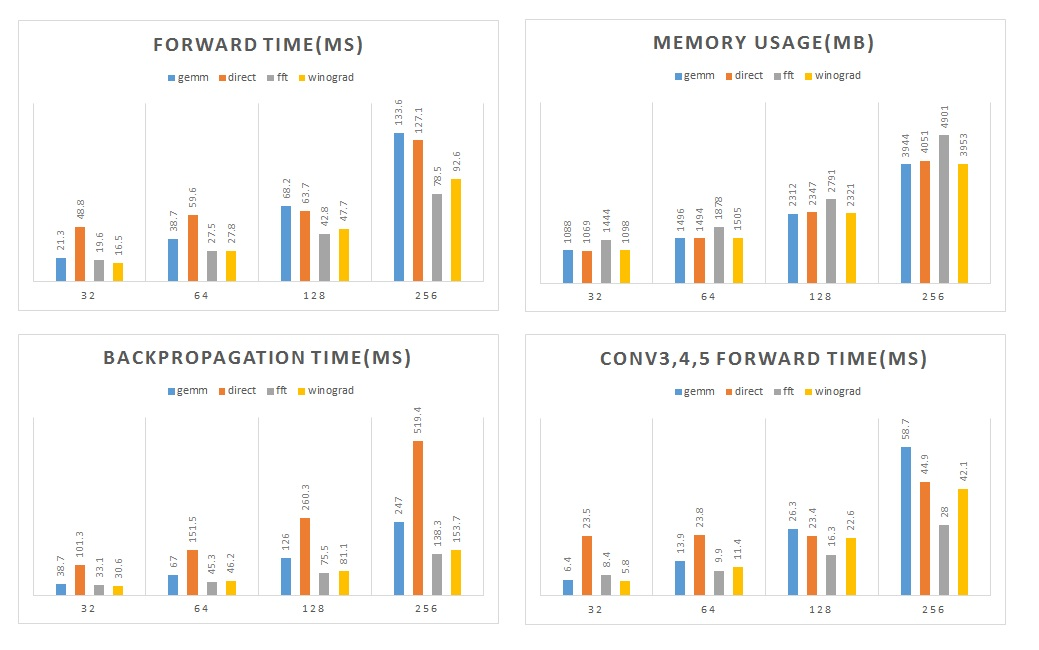
\includegraphics[width=\linewidth]{./figures/conv_time}
  \caption{Forward propagation and Backpropagation times of convolution algorithms. The times are measured as average of 100 batch iterations. 
Direct convolution is tested with cuda-convnet3 and other 3 are kernels of CuDNN R5. }
  \label{fig_conv_time}
\end{figure}

FIg \ref{fig_conv_time} shows execution time comparisons between convolution kernels.
Winograd convolution and FFT convolution always perform better than direct or gemm convolution, due to smaller floating point operations required.
FFT has smallest operations count, makes it fastest among algorithms on big batch inputs.
However FFT scales bad on smaller batch sizes because it executes 5 kernels per each layer.
The forward propagation speed comparison on conv layer 3,4,5 on (f) of Fig \ref{fig_conv_time} clearly shows the differences.
Cuda-convnet scales bad when the batch size is smaller than 128 while GEMM convolutoin sclaes almost linearly.
Winograd performs better when the batch size is smaller than 64, where theoretical operations per each layer is around 20G operations.
Winograd kernels are more efficient when the sample width is even.
When we increase the sample width of conv layer 3,4,5 from 13 to 14, the execution time of Winograd kernels decrease by 10\%.

Number of floating point operations needed for forward propagation and backward propagation kernels are equal on the same layer.
Therefore, execution time of forward and backward propagation kernels are almost symmetric on most convolution algorithms.
However, backpropagation kernels of direct convolution takes more execution time than their forward counterparts.
Especially backward filter convolution on first convolution layer takes 200ms to execute, occupying 40\% of total training time.
The reason for the slow execution is low parallelism of kernels.
The backward direct convolution kernels have small thread numbers compared to other algorithms, generating 6 times smaller thread grid size.
The backward filter convolution for the first layer generates only 1024 threads, while Titan X has 3072 CUDA cores.





\begin{figure}
  \centering
  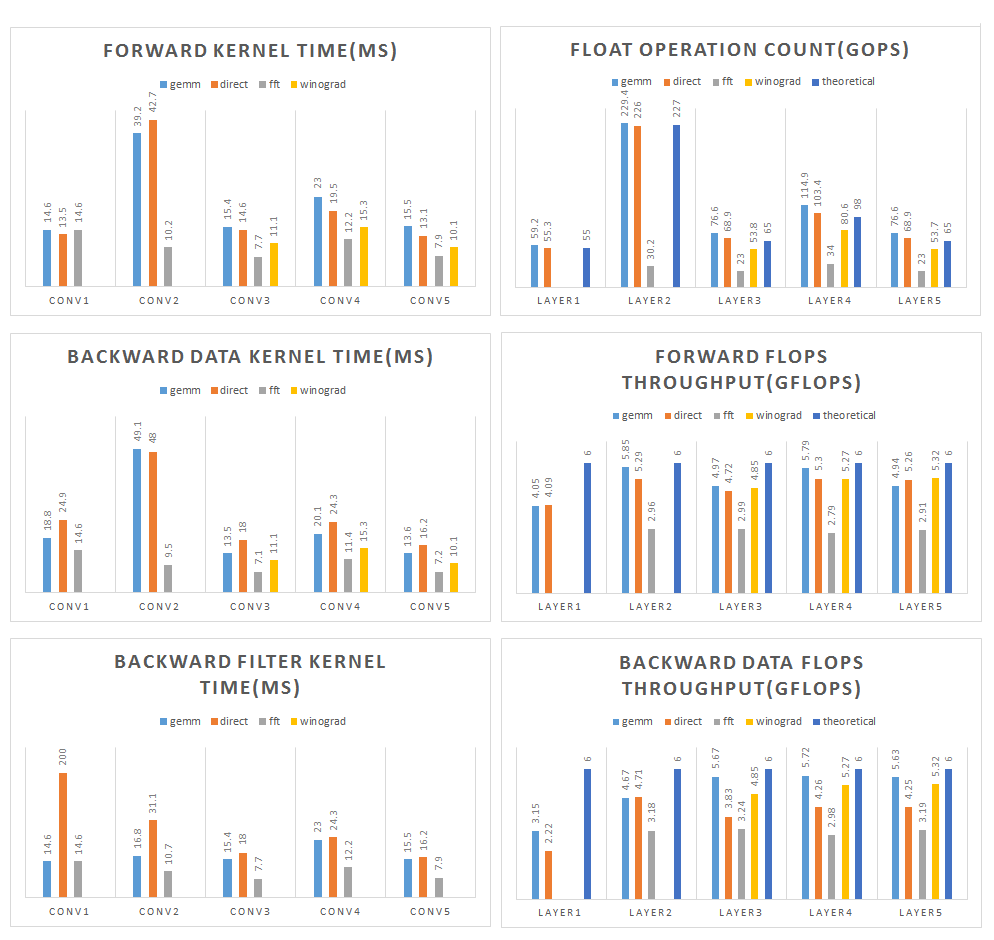
\includegraphics[width=\linewidth]{./figures/layerwise_bench}
  \caption{Layerwise analysis of convolution kernels}
  \label{fig_layerwise}
\end{figure}


\subsection{Multi GPU analysis}

\begin{itemize}
  \item Support
  \item Scalability : proportion of data exchange
  \item Synchronization cost
\end{itemize}

\section{Discussion / Conclusion}

\begin{itemize}
  \item Summary of results
  \item Compare frameworks : Implementation difference
  \item Locate bottleneck / suggest possible optimization
  \item Limitation, future research
\end{itemize}
